\documentclass[11pt]{llncs}
\usepackage{preamble}

\begin{document}
\import{./}{title.tex}
\thispagestyle{plain}
\import{./}{abstract.tex}
\import{./}{introduction.tex}
\import{./}{oracle.tex}

\section{Constructing non-interactive proofs}

A non-interactive proof-of-proof of work is a game between a Prover and a
Verifier parameterized by predicate $q$ which the prover tries to convience the
verifier for. The predicate $q$ is a function of a chain $\chain$, which the
prover claims to be the longest chain.

\import{./}{algorithms/alg.backbone.tex}
\import{./}{algorithms/alg.verifier-framework.tex}
\import{./}{algorithms/alg.verifier-full.tex}
\import{./}{algorithms/alg.verifier-lite.tex}

At the beginning of the game, two Provers generate proofs $\pi_A$, $\pi_B$
claiming potentially different truth values for the predicate $q$ based on
their claimed local longest chains. The Verifier receives these proofs and
accepts one of the two proofs, determining the truth value of the predicate.

We say that a predicate $q$ is $\textit{reliable}$ if it has the following
desirable properties:

\begin{itemize}
    \item The predicate is $\textit{monotonous}$ for honest provers: For a
        sequence of chains $\chain _1, \chain _2, \ldots$ of an honest prover, we
        have the there is some $i$ such that the predicate $q(\chain _j)$ is
        false for all j before that i; and subsequently, the predicate
        $q(\chain _j)$ becomes true for $j \geq i$ and remains true for ever.
        It is legal for $i$ to be at infinity, making the predicate false
        throughout.
    \item The predicate has $\textit{liveness}$: Once the environment puts
        adequate data in the blockchain payload for the predicate to become
        true, it will become true for all honest players.
    \item The predicate has $\textit{common prefix}$: Once it becomes true for
        one honest player, the rest will eventually follow.
\end{itemize}

\import{./}{algorithms/alg.nipopow-innerchain.tex}

We introduce a helper algorithm, ConstructInnerChain, shown in
Algorithm~\ref{alg.nipopow_construct_innerchain}. This algorithm returns the innerchain
of level $i$ extracted from the blockchain $\chain$. If boundary is provided,
it only returns the blocks more recent than the boundary block supplied.

\import{./}{algorithms/alg.nipopow-prover.tex}

The NiPoPoW proof construction is shown in Algorithm~\ref{alg.nipopow_construct_proof}.
This produces a non-interactive PoPoW in parameter $m$ which consists of a
number of blocks for every level $i$. The number of blocks per level is
approximately $2m$.

\begin{figure}[h]
    \caption{The hierarchical blockchain. Existing blocks are shown in level 1.
    Higher levels have achieved a lower target (higher difficulty) during mining.}
    \centering
    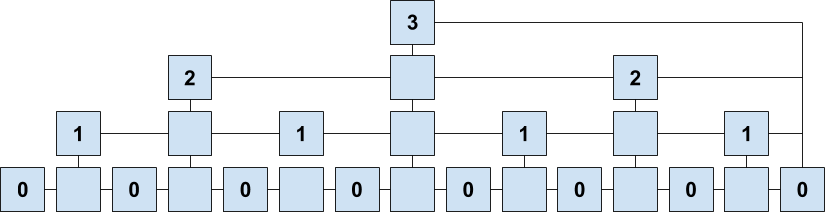
\includegraphics[width=\textwidth,keepaspectratio]{figures/hierarchical-ledger.png}
    \label{fig:hierarchy}
\end{figure}

\begin{figure}[h]
    \caption{The first of a series of interactive proofs-of-proofs-of-work for
    $m = k = 3$. This proof is the only one that needs to be sent in case it
    goes unchallenged.}
    \centering
    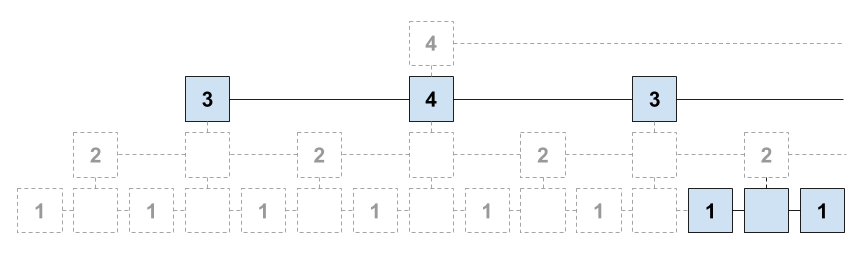
\includegraphics[width=\textwidth,keepaspectratio]{figures/interactive-popow.png}
\end{figure}

\begin{figure}[h]
    \caption{A non-interactive proof-of-work for $m = k = 3$. Any challenges
    can be answered by the verifier directly by constructing a proof from the
    data in this proof, without interaction with the prover.}
    \centering
    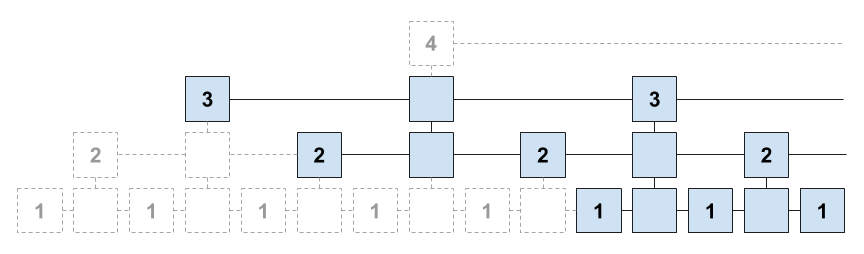
\includegraphics[width=\textwidth,keepaspectratio]{figures/non-interactive-popow.png}
\end{figure}

\import{./}{references.tex}
\end{document}
